\documentclass[journal,onecolumn,]{IEEEtran}

% Packages
\usepackage{times}
\usepackage[pdftex]{graphicx}
\usepackage{amsmath,amssymb,amsopn,amstext,amsfonts}
\usepackage{cancel}
\usepackage[space]{cite}
\usepackage{pdfsync}
\usepackage{balance}
\usepackage{color}
\usepackage{mathtools}
\usepackage{algpseudocode}
\usepackage{algorithm} %\usepackage[ruled,vlined,linesnumbered]{algorithm2e}
\usepackage{bm}
\newtheorem{theorem}{Theorem}
\usepackage{diagbox}
\usepackage{float}
\usepackage{epstopdf}
\usepackage{pifont}
\usepackage{amsmath}
\usepackage{multirow}
\usepackage{url}
\usepackage{verbatim}
\usepackage[linkcolor=black,citecolor=black,urlcolor=black,colorlinks=true]{hyperref}
%\usepackage{enumitem}
\usepackage{booktabs}
\usepackage{graphicx}
\usepackage{subcaption}
\usepackage{threeparttable}  
\usepackage{orcidlink}

\usepackage{algorithm}

\ifCLASSINFOpdf

\title{AWP Token: Bridging CS2 Culture \\ with the Crypto World}
\author{AWP Comunication \\ https://awp-gg.xyz/}
\date{}


	
\usepackage{titlesec}
\titleformat{\section}[block]{\normalfont\Large\bfseries\filright}{\thesection}{1em}{}
\titleformat{\subsection}[block]{\normalfont\large\bfseries\filright}{\thesubsection}{1em}{}
\titleformat{\subsubsection}[block]{\normalfont\normalsize\bfseries\filright}{\thesubsubsection}{1em}{}

\begin{document}
	
	\maketitle
	
	\section*{Abstract}
	As cryptocurrencies become increasingly important in societal transactions and structures, Arctic Warfare Police(AWP) Token has emerged to bring the unique culture of the Counter-Strike2(CS2) community into the crypto world. Inspired by the famous AWP sniper rifle in CS2, the AWP Token is not just a cryptocurrency but also a tribute to AWP culture and the CS2 community. Although the AWP Token does not pursue economic value, it provides a new way of social and cultural exchange for CS2 players and cryptocurrency enthusiasts. 
	
	\section{Introduction}
	
	The AWP is a well-known sniper rifle in CS2\cite{CSGOBombCode}, beloved by players for its powerful firepower and precision. More than just a weapon, it has become a symbol of skill and honor within the gaming community. Its iconic ability to deliver a one-shot kill at long distances plays a pivotal role in competitive matches and has become a cultural icon for players and fans alike.
	
	The AWP Token is designed to merge players' passion for AWP culture\cite{PixelsUnderstandingSignificance} with the world of cryptocurrencies, creating a conduit between the adrenaline-driven arenas of esports and the innovative sphere of digital currencies. As a blockchain-based meme coin, it is not a traditional investment vehicle but a cultural token that conveys recognition and respect for the AWP culture within CS2. It offers community members a way to share and celebrate the thrilling moments that happen in the game.
	
	Furthermore, the launch of the AWP Token is about reinforcing a shared identity and a sense of belonging among CS2 enthusiasts worldwide. It eschews financial transactions to emphasize the cultural and community connections, thereby deepening social interaction both within and outside the game.
	
	By integrating with the world of cryptocurrencies, the AWP Token introduces an innovative mode of community participation\cite{nakamotoBitcoinPeertoPeerElectronic}. It captures the excitement around CS2 and transforms it into a new social and cultural experience, encouraging players to share their gaming experiences and strengthening the bonds within the gaming community.
	
	As the AWP Token evolves, it strives to encapsulate the essence of CS2's competitive spirit in each cultural exchange. It serves as a recognition of the dedication of those who spend hours honing their skills and the strategists who deftly outmaneuver their opponents. The AWP Token symbolizes an evolution in gaming culture and an intriguing blend with the culture of cryptocurrencies.



	\section{Supply and Initial Distribution}
	The total supply of AWP Tokens is set at \textbf{1,000,022} to commemorate the unique status of the AWP in CS2. This supply is fixed and will not increase, maintaining its scarcity and value. Initial liquidity is provided by the project's founders to ensure the market liquidity of the AWP Token.
	
		
	AWP Token contract address: 
	
	\begin{itemize}
		\item 	\textbf{0x5e9fE073Df7Ce50E91EB9CBb010B99EF6035a97D}
	\end{itemize}
	
	The tokens held by the team have been transferred and are protected by a multi-signature wallet on the Base chain with an execution threshold of \textbf{3/4}.
	
	 Multi-signature wallet address: 
	 
	 	\begin{itemize}
	 	\item 	\textbf{0xDf8818C289e863b614Ed04938ba41220c7fA74F8}
	 \end{itemize}
	 
	  

	
	 
	
	\section{Logo and Base Chain}
	The logo of the AWP Token adopts the classic AWP sniper rifle from CS2, symbolizing respect and love for this weapon, show as Fig.\ref{pic:1} The Base chain is chosen to launch the AWP Token, aiming to utilize its efficiency and accessibility, while expressing respect for the Ethereum chain as the birthplace of cryptocurrencies.
	
	
	
		\begin{figure*}[h]
		\centering
		\begin{subfigure}{0.45\linewidth}
			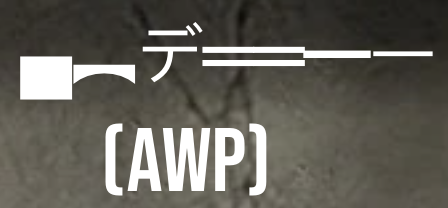
\includegraphics[width=1\linewidth]{figure/1.png}
			\captionsetup{font={small}}
			\caption{AWP Token logo}
			\label{pic:12}
		\end{subfigure}
		\begin{subfigure}{0.45\linewidth}
			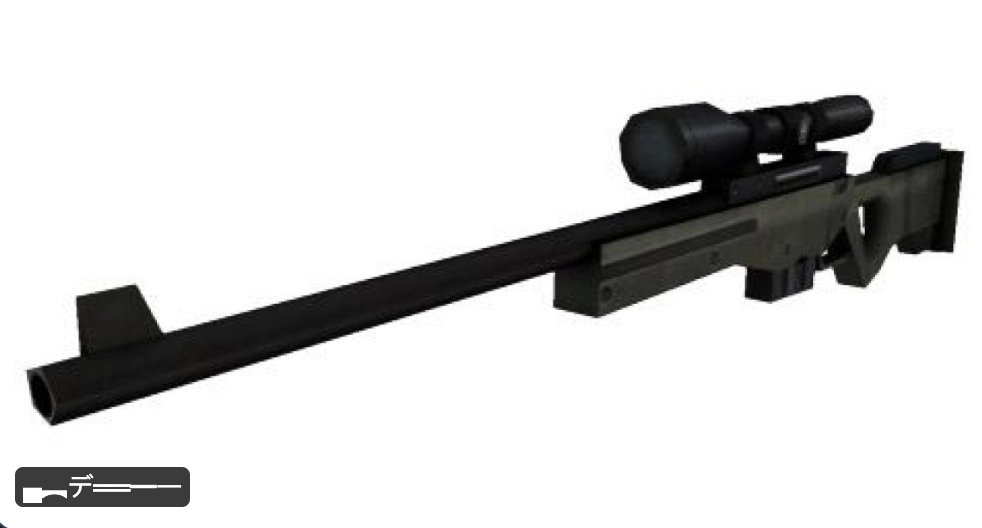
\includegraphics[width=1\linewidth]{figure/3.png}
			\captionsetup{font={small}}
			\caption{Physical representation of the AWP in CS2}
			\label{pic:11}
		\end{subfigure}
		\captionsetup{font={small}}
		\caption{
			AWP Cultural Mapping. a) The logo for the AWP Token, featuring design elements that incorporate the silhouette of the AWP sniper rifle, reflective of the token's connection to the gaming community. b) A detailed depiction of the AWP sniper rifle from Counter-Strike: Global Offensive, highlighting its distinctive scope, barrel, and stock, symbolic of its power and precision within the game. }
		\label{pic:1}
		\vspace{-0.5cm}
	\end{figure*}
	
	
	\section{Supply Adjustment}
	To demonstrate a long-term commitment to the project, the project initially destroyed the provided liquidity certificates. With 
	
	Transaction Hash:
	
		\begin{itemize}
		\item 	\textbf{0x6ad33cea6a9a8743eebd87e73aa3fd33b1a6454977c51ac428fef747945215bc}
	\end{itemize}



	Subsequently, to reduce the circulating supply and enhance community trust, multiple supply destruction operations were carried out, totaling \textbf{16.5\%} of the supply. With
	
	Transaction Hashes are:
	
	\begin{itemize}
		\item \textbf{0xfc487c0d7996e64fde72c9ae16defddc7c17b08ce599da7d975de7ecc1012f36}
		\item \textbf{0x4bf1c3f7c347c6a52aed57dc17340549febf1edc882988c11c2c0ca3ed19bae3}
		\item \textbf{0x015f3b7f2e65d1f40d45d00c0c9f91d3ce5ca8e776f2dc09347631366efde60d}
	\end{itemize}
	
	\section{Conclusion}
	The launch of the AWP Token is a tribute to the AWP sniper rifle culture in CS2. It is not only a cryptocurrency but also a cultural symbol. It provides a platform for CS2 players and cryptocurrency enthusiasts to communicate and resonate, promoting the spread and development of AWP culture in the crypto world.
	
	
	\section*{Disclaimer}

			AWP Token is a tribute to the AWP sniper rifle culture in CS2, and it is not designed for profit. The information provided in this article does not constitute financial advice. If you are interested in AWP Token, feel free to participate; if not, that is perfectly fine. If you do not believe or understand, we kindly ask for your understanding, as we may not be able to invest time in detailed explanations.
		
		
	\vfill
	
	\bibliographystyle{IEEEtran} 
	\bibliography{awp2024}


	
	\vfill
		
\end{document}
